\documentclass[12pt]{fphw}

% Template-specific packages
\usepackage[utf8]{inputenc} % Required for inputting international characters
\usepackage[T1]{fontenc} % Output font encoding for international characters
\usepackage{mathpazo} % Use the Palatino font
\usepackage{alphabeta} % Use the Palatino font
\usepackage{graphicx} % Required for including images
\usepackage{booktabs} % Required for better horizontal rules in tables
\usepackage{listings} % Required for insertion of code
\usepackage{enumerate} % To modify the enumerate environment
\usepackage{hyperref}
\usepackage{graphicx}
\usepackage{amsmath}
\graphicspath{{./images/}}
\usepackage{framed} % or, "mdframed"
\usepackage[framed]{ntheorem}
\usepackage{amssymb}
\usepackage{xcolor}
\usepackage{tabularx}

\newframedtheorem{frm-thm}{Theorem}
% \newtheorem{theorem}{Theorem}
\usepackage{tikz} 
\hypersetup{
    colorlinks=true,
    linkcolor=blue,
    filecolor=magenta,      
    urlcolor=cyan,
}
\urlstyle{same}
%----------------------------------------------------------------------------------------
%	ASSIGNMENT INFORMATION
%----------------------------------------------------------------------------------------

\title{Deep Learning for NLP} % Assignment title
\author{{Μπαρμπαρόσος Θεοφάνης} \\sdi: {sdi2200107}} % Student id
\date{Spring Semester 2025} % Due date
\institute{University of Athens \\ Department of Informatics and Telecommunications} % Institute or school name
\class{Artificial Intelligence II (M138, M226, M262, M325) } % Course or class name
%----------------------------------------------------------------------------------------
\begin{document}
\maketitle % Output the assignment title, created automatically using the information in the custom commands above
%----------------------------------------------------------------------------------------
%	ASSIGNMENT CONTENT
%----------------------------------------------------------------------------------------

{
  \hypersetup{linkcolor=black}
  \tableofcontents
}
\newpage

\section{Abstract}
In this project, we developed a sentiment analysis classifier using Logistic Regression and TF-IDF feature extraction on an English-language Twitter dataset. The primary objective is to design an effective text classification model that can accurately predict the sentiment of a tweet as either positive or negative. This task involves several key steps, including exploratory data analysis, data preprocessing, feature extraction, model training, and evaluation using various performance metrics.

\section{Data processing and analysis}

\subsection{Exploratory Data Analysis}
In this first part of the project, I performed an Exploratory Data Analysis(EDA) of the given data, specifically, regarding both the training and the validation datasets. This process aims to provide a better view of the datasets as, through plots and various statistics we are able to better understand their composition.{\newline}
\begin{enumerate}
    \item Initially, the first 5 entries of each dataset are displayed as a brief sample of the dataset, along with some basic information describing the whole dataset such as, total number of entries, the different data types that make up each record etc.(Figure 1)
    \begin{figure}[h]
        \begin{center}
            \caption{}
            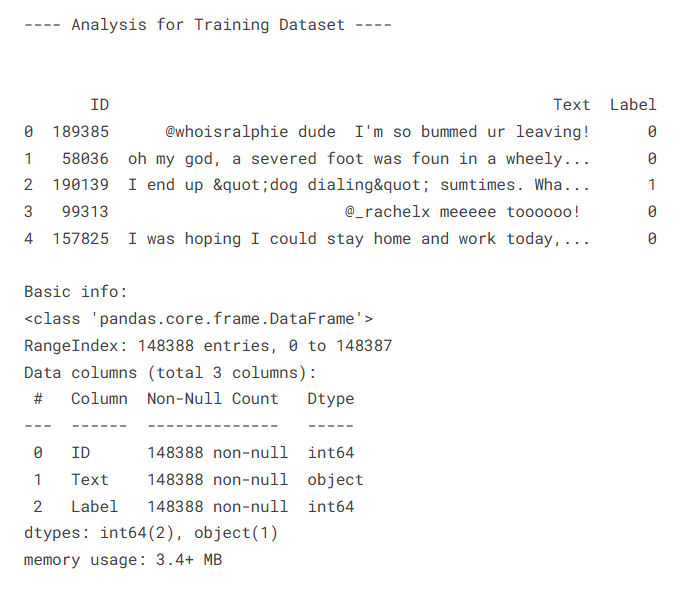
\includegraphics[scale=0.7]{screenshot.png}
        \end{center}
    \end{figure}
    \pagebreak
    
    \item Plots are printed to showcase the length distribution of tweets both in characters count and in words count. (Figures 2 \& 3)
    \begin{figure}[h]
        \begin{center}
            \caption{}
            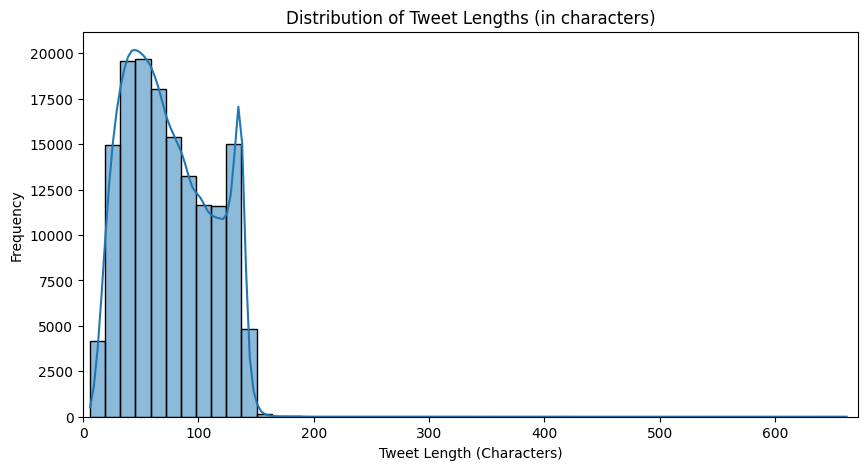
\includegraphics[scale=0.65]{__results___2_2.png}
        \end{center}
    \end{figure}
    \begin{figure}[h]
        \begin{center}
            \caption{}
            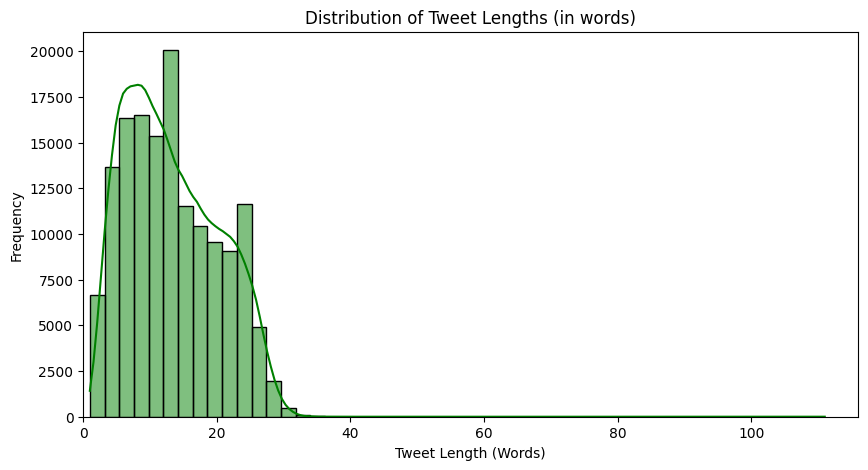
\includegraphics[scale=0.65]{__results___2_4.png}
        \end{center}
    \end{figure}
    \pagebreak
    
    \item A plot is printed to showcase the number of punctuation marks in tweets per label. (Figure 4)
    \begin{figure}[h]
        \begin{center}
            \caption{}
            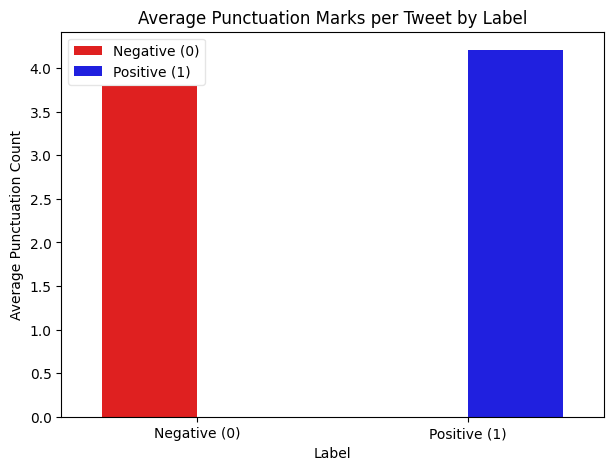
\includegraphics[scale=1]{__results___2_6.png}
        \end{center}
    \end{figure}{\newline\newline\newline}
    
    \item A plot (alongside exact numbers) is printed to showcase the distribution of tweets per label. (Figure 5)
    \begin{figure}[h]
        \begin{center}
            \caption{}
            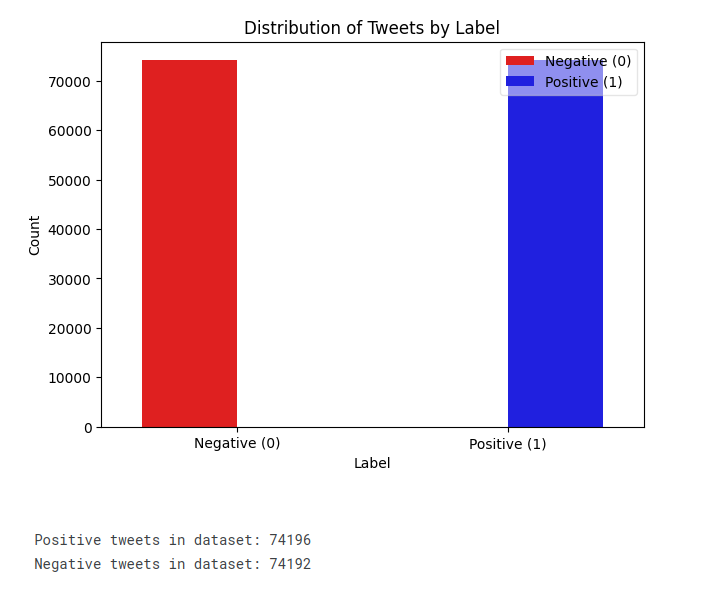
\includegraphics[scale=0.7]{screenshot1.png}
        \end{center}
    \end{figure}
    \pagebreak
    \item Lastly, two plots are printed to showcase the number of correctly spelled words (Figure 6) and the number of misspelled words (Figure 7) in tweets per label.
    \begin{figure}
        \begin{center}
            \caption{}
            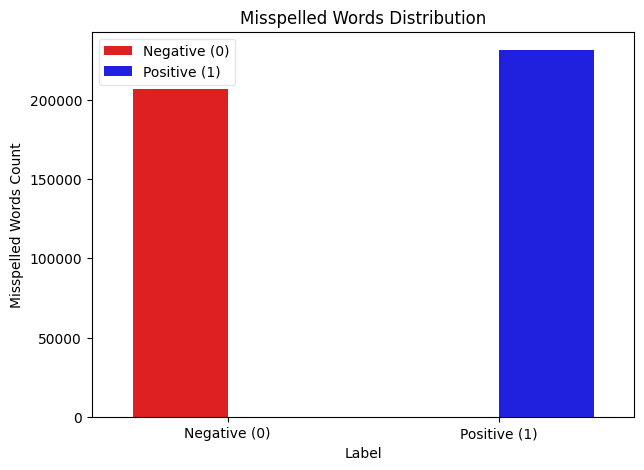
\includegraphics[scale=0.9]{__results___2_11.png}
        \end{center}
    \end{figure}
    \begin{figure}
        \begin{center}
            \caption{}
            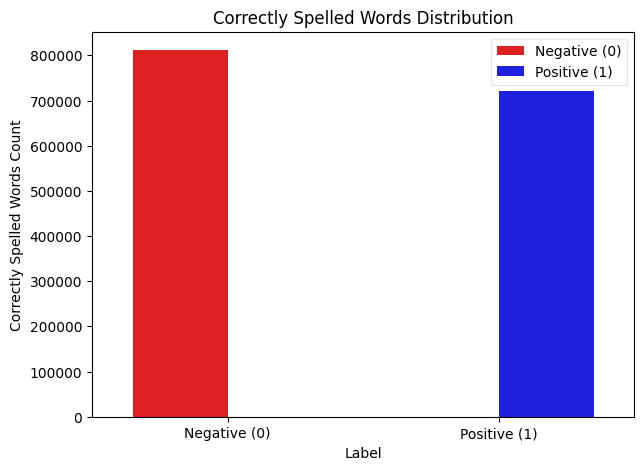
\includegraphics[scale=0.9]{__results___2_13.png}
        \end{center}
    \end{figure}
\end{enumerate}
\pagebreak
As mentioned before, the EDA described above, is performed on both the training and the validation datasets.
(specific plots and outputs refer to the training dataset as an example)

\subsection{Pre-processing}

In this step, I implemented multiple preprocessing techniques to clean and normalize the Twitter dataset, ensuring it was suitable for feature extraction and classification. The following methods were applied:
\begin{enumerate}
    \item \textbf{Lowercasing}: All text was converted to lowercase to ensure consistency and eliminate redundancy in token representation.
    \item \textbf{Replacing Emails, URLs, and Mentions}: Using regular expressions, email addresses were replaced with the token "email", URLs with "url", and Twitter mentions (e.g., @username) were removed, as they do not contribute to sentiment analysis.
    \item \textbf{Handling Hashtags}: Hashtags were processed by removing the "\#" symbol while preserving the associated word (e.g., "\#happy" becomes "happy").
    \item \textbf{Removing Ellipses}: Consecutive dots (e.g., "...", "....", ".....") were replaced with a single space to normalize punctuation usage.
    \item \textbf{HTML Entity Decoding}: HTML-encoded characters were converted to their corresponding textual representation (e.g., "\&amp;" becomes "\&").
    \item \textbf{Handling Repeated Characters}: Words with unnecessarily long character repetitions were normalized by limiting repetitions to at most two occurrences (e.g., "soooo" becomes "soo").
    \item \textbf{Expanding Contractions}: Common English contractions were expanded to their full forms (e.g., "haven't" becomes "have not") to enhance textual clarity and standardization.
    \item \textbf{Removing Non-Alphanumeric Characters}: Any character that is not an English letter, number, or whitespace was removed to eliminate noise and improve text quality.
    \item \textbf{Spell Checking}: A spell checker (e.g., PySpellChecker) was applied to correct misspelled words, ensuring more accurate text representation.
\end{enumerate}

After applying these preprocessing techniques, the cleaned text was ready for feature extraction using TF-IDF. The cleaned dataset significantly improved classification performance by reducing irrelevant features and enhancing meaningful word representations.{\newline}

The set of techniques mentioned above, in this specific order, is a choice conducted upon extensive testing and experimenting with various preprocessing methods.\pagebreak

\subsection{Data partitioning for train, test and validation}
The data for the project as a whole is partitioned in three datasets with the same structure: a training dataset, a validation dataset and a test dataset. Exploratory Data Analysis is performed on the training and validation datasets only as the test dataset is theoretically not given and it is used without ever knowing specifically what it contains. All three datasets unergo the same preprocessing as discussed previously. The model is then trained on the training dataset and is tested and evaluated on the validation dataset. Finally, a prediction result is produced for the test dataset which is used primarily for the Kaggle submission.

\subsection{Vectorization}

In this task, the \textbf{TF-IDF(Term Frequency-Inverse Document Frequency)} method was applied to convert textual data into numerical representations that are suitable for machine learning models.

\subsubsection{Understanding TF-IDF}

TF-IDF is a statistical approach used to determine the significance of a word in a document relative to an entire collection of documents. It highlights terms that appear frequently in a specific document but are uncommon across the dataset, allowing the model to focus on meaningful and distinctive words.

\subsubsection{TF-IDF Mechanism}

TF-IDF is composed of two key elements:

\begin{itemize}
    \item \textbf{Term Frequency (TF):} Quantifies how often a word occurs in a document.
    \[
    \text{TF}(t, d) = \frac{\text{Number of times term t appears in document d}}{\text{Total number of terms in d}}
    \]
    \item \textbf{Inverse Document Frequency (IDF):} Assesses the significance of a word across the entire document set.
    \[
    \text{IDF}(t) = \log \left( \frac{N}{DF(t)} \right)
    \]
    where $N$ represents the total number of documents, and $DF(t)$ denotes the number of documents containing the term $t$. The logarithm helps prevent highly frequent words from dominating the score.
\end{itemize}

The TF-IDF score is then computed as:
\[
\text{TF-IDF}(t, d) = \text{TF}(t, d) \times \text{IDF}(t)
\]

\subsubsection{Why Use log in IDF?}

The logarithmic function is used to ensure that extremely common words (such as "the" or "is") do not disproportionately affect the weighting. Without logarithmic scaling, the variance in IDF values would be significantly larger, leading to an unbalanced representation of term importance.

\subsubsection{Limitations of TF-IDF}

While TF-IDF is a powerful technique, it has certain drawbacks:
\begin{itemize}
    \item It does not capture semantic relationships—synonyms like "happy" and "joy" are treated as unrelated words
    \item It disregards word order and phrases—terms such as "machine learning" are processed as independent words.
    \item It may assign excessive importance to rare words, even if they are irrelevant or misspelled.
    \item It does not differentiate between distinct meanings of the same word (e.g., "Apple" as a fruit versus "Apple" as a company).
\end{itemize}


\section{Algorithms and Experiments}

\subsection{Experiments}

To tackle the sentiment analysis problem, I started by experimenting with various preprocessing techniques to clean up the text data before training the model. Initially, I applied basic text-cleaning methods such as lowercasing and removing non-alphanumeric characters. However, I progressively refined my approach by testing more advanced techniques and analyzing their impact on model accuracy.\newline\newline
\textbf{Preprocessing Trials}
\begin{itemize}
    \item \textbf{Stopwords Removal:} Contrary to common practice, removing stopwords decreased accuracy. Keeping stopwords led to better performance, likely because they contribute contextual information in sentiment analysis.
    
    \item \textbf{Spell Checking:} I tested multiple spell-checking methods:
    \begin{itemize}
        \item Using an extensive dictionary with a wide range of possible misspellings did not significantly improve accuracy. Additionally, this approach is inefficient and will likely lead to overfitting.
        \item TextBlob and SymSpell were both tested but did not result in better accuracy and ultimately opted for pyspellchecker to perform spell checking on the data.
        \item Spell checking with \texttt{distance=2} in the SpellChecker library was too slow (>30 minutes).
        \item A hybrid spell-checking approach was also tested: first, all words were corrected using \texttt{distance=1}, and for words without corrections, \texttt{distance=2} was applied. However, this was still too slow and did not improve accuracy.
    \end{itemize}
    
    \item \textbf{Lemmatization \& Stemming:} Both techniques unexpectedly reduced accuracy, likely due to the loss of important word forms that carry sentiment nuances.

    \item \textbf{Slang Normalization:} I attempted replacing common slang terms with their full equivalents. However, this approach reduced accuracy. The following function and dictionary was used:

    \begin{verbatim}
    def remove_slang(text):
        slang = {
            "gr8": "great", "gud": "good", "bbq": "barbeque",
            "btw": "by the way", "4all": "for all", "yeah": "yes",
            "cuz": "because", "coz": "because", "dis": "this",
            "dat": "that", "y'all": "you all", "nah": "no",
            "nope": "no", "omg": "oh my god", "thankz": "thanks",
            "btwn": "between", "cpl": "couple", "ty": "thank you",
            "imo": "in my opinion", "brb": "be right back",
            "ttyl": "talk to you later",
            "imho": "in my honest opinion",
            "fyi": "for your information", "tbh": "to be honest",
            "nvm": "nevermind", "w/o": "without",
            "wyd": "what are you doing", "ikr": "I know, right?",
            "ez": "easy", "prolly": "probably",
            "gimme": "give me", "lemme": "let me", "thanx":
            "thanks", "dunno": "do not know",
            "lmk": "let me know", "2night": "tonight",
            "2morrow": "tomorrow", "b2b": "back to back",
            "cya": "see you", "ya": "you", "lol": "laugh out loud",
            "lmao": "laughing my ass off",
            "lmfao": "laughing my fucking ass off",
            "rofl": "rolling on the floor",
            "roflmao": "rolling on the floor laughing my ass off",
            "streetz": "streets", "telly": "television",
            "tv": "television"
        }
        for wrong, correct in slang.items():
            text = re.sub(rf"\b{re.escape(wrong)}\b", correct, text)
        return text
    \end{verbatim}

    When increasing the \texttt{n\_gram\_range} to (1,3) or (1,4), the negative impact of slang normalization was slightly reduced, but overall, avoiding slang replacement produced better accuracy.

    \item \textbf{Handling Time Expressions:} I experimented with the following regex pattern to normalize time expressions like "1030pm" to "1030 pm":   \begin{verbatim}
        text = re.sub(r'(\d+)([ap]m)', r'\1 \2', text)
    \end{verbatim}
    However, this preprocessing step led to a decrease in accuracy.

\end{itemize}

These trials highlight how different preprocessing techniques can significantly impact model performance. Some intuitive choices, such as lemmatization and slang normalization, unexpectedly reduced accuracy. The best results were achieved by retaining stopwords, avoiding excessive spell-checking, and carefully tuning text normalization techniques.

\subsection{Hyper-parameter tuning}

In order to optimize the performance of the Logistic Regression model, I manually experimented with various hyperparameters rather than utilizing tools like Grid Search, as it was computationally expensive and time-consuming.

The key hyperparameters I tuned were:
\begin{itemize}
    \item \textbf{ngram\_range}: I tested different values, including (1,2), (1,3), (2,3), (1,4), (1,5) and (1,6). The best results were obtained with (1,4), as it captured both individual words and meaningful phrases.
    \item \textbf{max\_features}: After experimenting with values ranging from 1,000 to 1,000,000, I selected 100,000 as a balanced choice between performance and computational efficiency.
    \item \textbf{min\_df and max\_df}: Setting \texttt{min\_df=3} and \texttt{max\_df=0.9} helped filter out overly rare and overly common words, improving generalization.
    \item \textbf{Random State}: A fixed \texttt{random\_state=161} was used to ensure reproducibility.
\end{itemize}

The model was monitored for overfitting and underfitting:
\begin{itemize}
    \item A very high training accuracy but poor validation accuracy indicated overfitting, which was mitigated by adjusting \texttt{max\_df} and restricting the feature set.
    \item A low training accuracy indicated underfitting, which was improved by increasing \texttt{max\_features} and tuning the \texttt{ngram\_range}.
\end{itemize}

\subsection{Optimization techniques}

To further enhance model performance and training efficiency, the following optimization techniques were applied:
\begin{itemize}
    \item \textbf{TF-IDF Weighting}: This technique ensured that words significant for classification were appropriately weighted, reducing the influence of frequently occurring but uninformative terms.
    \item \textbf{Feature Selection}: By limiting \texttt{max\_features} and adjusting \texttt{min\_df}, I removed noise from the dataset, improving generalization.
    \item \textbf{Regularization}: Logistic Regression inherently applies L2 regularization (Ridge), which helps in preventing overfitting by penalizing large coefficients.
    \item \textbf{Efficient Data Handling}: Sparse matrices were used to store TF-IDF vectors, reducing memory consumption and computational load.
\end{itemize}

These optimizations helped stabilize training and improved overall model robustness.

\subsection{Evaluation}

The model's performance was assessed using standard evaluation metrics:
\begin{itemize}
    \item \textbf{Accuracy}: Measures overall correctness of predictions.
    \item \textbf{Precision, Recall, and F1-score}: Provides insights into false positives and false negatives.
    \item \textbf{Confusion Matrix}: Visualizes model misclassifications.
    \item \textbf{ROC Curve}: Evaluates the trade-off between true positive and false positive rates.
\end{itemize}

\subsubsection{ROC Curve}
The ROC (Receiver Operating Characteristic) curve illustrates the true positive rate against the false positive rate at various threshold levels. A higher AUC (Area Under the Curve) score indicates a better-performing model. The ROC curve is shown in Figure 8.

\subsubsection{Learning Curve}
The learning curve showcases training vs. validation accuracy over iterations. If there is a large gap between the two, it indicates overfitting. A properly tuned model should show convergence between these curves. (Figure 9)

\subsubsection{Confusion Matrix}
The confusion matrix (Figure 10) provides a breakdown of correct and incorrect predictions. It helps analyze where the model struggles (e.g., misclassifying positive sentiment as negative).

The matrix is as follows:
\begin{equation}
    \begin{bmatrix}
        TP & FN \\
        FP & TN
    \end{bmatrix}
\end{equation}
Where:
\begin{itemize}
    \item \textbf{TP (True Positives)}: Correctly predicted positive sentiments.
    \item \textbf{FN (False Negatives)}: Positive sentiments misclassified as negative.
    \item \textbf{FP (False Positives)}: Negative sentiments misclassified as positive.
    \item \textbf{TN (True Negatives)}: Correctly predicted negative sentiments.
\end{itemize}
Analysis of these evaluation metrics, ensured model reliability and identified areas for further improvement.

\begin{figure}
    \begin{center}
        \caption{}
        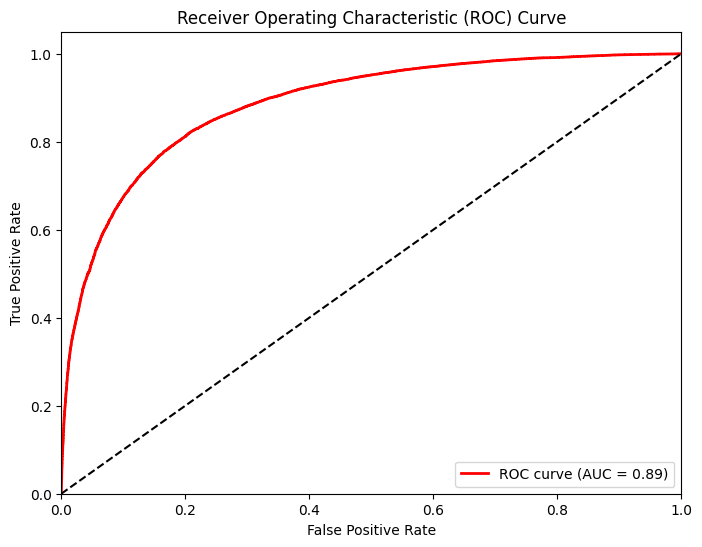
\includegraphics[scale=0.9]{roc.png}
    \end{center}
\end{figure}

\begin{figure}
    \begin{center}
        \caption{}
        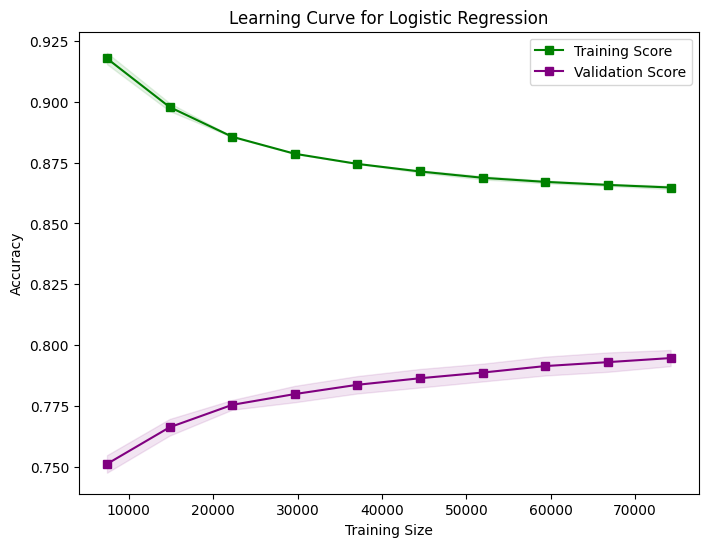
\includegraphics[scale=0.83]{learning curves.png}
    \end{center}
\end{figure}

\begin{figure}
    \begin{center}
        \caption{}
        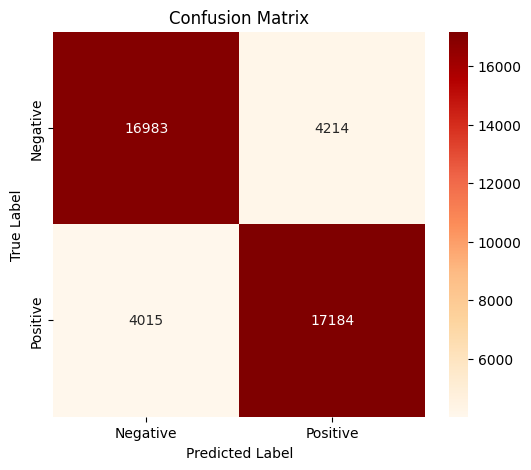
\includegraphics[scale=0.83]{conf_matrix.png}
    \end{center}
\end{figure}

\pagebreak

\section{Results and Overall Analysis}

\subsection{Results Analysis}

The results of the project were both expected and somewhat surprising. While some outcomes were anticipated, some aspects did not align with our expectations. Specifically, some features I thought would improve the model’s accuracy, actually had the opposite effect. As a result, various techniques were applied. Some of which improved performance as expected, while others did not, prompting further analysis and exploration of the model’s decision-making process. This, in turn, led to a deeper understanding of what truly enhances the model and what does not.{\newline}
Throughout this report, accuracy values are omitted because testing was performed locally. Therefore, specific numbers would not provide much useful information as the testing dataset and machine would ultimately differ from mine. Nonetheless, here are some results showcasing the process followed at various experimenting stages:
\begin{enumerate}
    \item Only text lowercasing and the default arguments in the TfidfVectorizer() function call and only random\_state=161 for the LogisticRegression(random\_state=161): (Figure 11)
    \item Full pre processing with all the pre processing techniques and all the hyperparameters discussed before: (Figure 12)
\end{enumerate}
\pagebreak
\begin{figure}
    \begin{center}
        \caption{}
        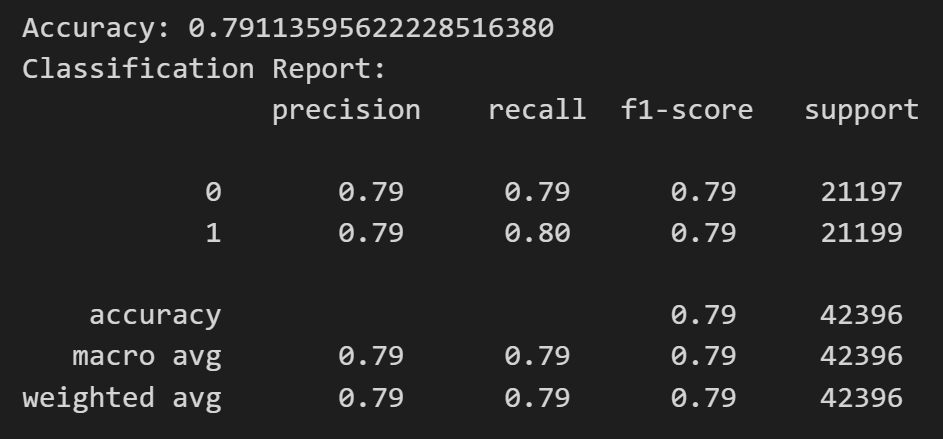
\includegraphics[scale=0.6]{Στιγμιότυπο οθόνης 2025-03-29 133856.png}
    \end{center}
\end{figure}
\begin{figure}
    \begin{center}
        \caption{}
        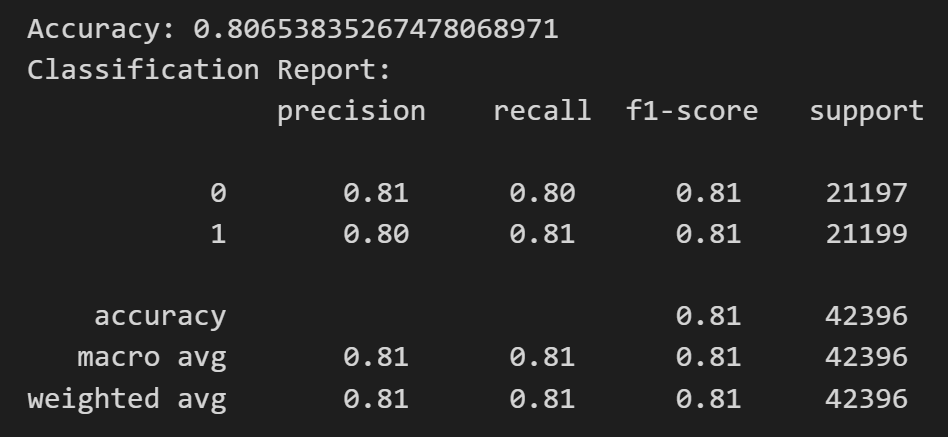
\includegraphics[scale=0.6]{Στιγμιότυπο οθόνης 2025-03-29 133602.png}
    \end{center}
\end{figure}


\subsubsection{Best trial}

My final, best trial is the one submitted to the competition. It incorporates all the preprocessing techniques specified in section 2.2 of this report, as well as all the hyperparameters for the TfidfVectorizer() and LogisticRegression() outlined in section 3.3. This combination of methods represents the optimal approach, ensuring the best possible text preparation and the most fine-tuned model training. Results from this trial (tested on the validation dataset and on my machine) are shown in Figure 12. However, as mentioned earlier, this is not entirely indicative of the actual performance on the competition platform. The final results I obtained on Kaggle are shown in Figure 13, with the best accuracy on the test dataset reaching 0.80484.
\begin{figure}
    \begin{center}
        \caption{}
        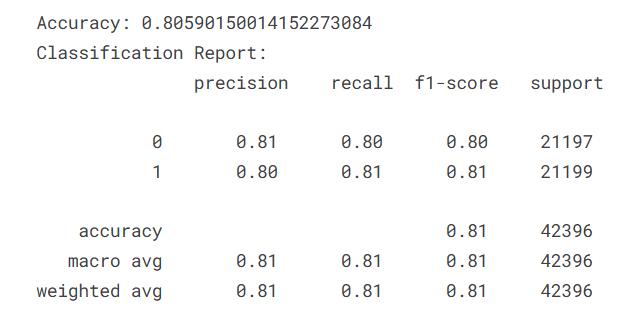
\includegraphics[scale=0.9]{Στιγμιότυπο οθόνης 2025-03-29 135645.png}
    \end{center}
\end{figure}
\pagebreak

\subsection{Comparison with the first project} 

\addwhenneeded{Use only for projects 2,3,4}\\
\instructornote{Comment the results. Why the results are better/worse/the same?}

\subsection{Comparison with the second project}

\addwhenneeded{Use only for projects 3,4}\\
\instructornote{Comment the results. Why the results are better/worse/the same?}

\subsection{Comparison with the third project}

\addwhenneeded{Use only for project 4}\\
\instructornote{Comment the results. Why the results are better/worse/the same?}


\section{Bibliography}

\bibliographystyle{plain} % We choose the "plain" reference style
\bibliography{refs} % Entries are in the refs.bib file

\instructornote{You should link and cite whatever you used or "got inspired" from the web. Use the /\ cite command and add the paper/website/tutorial in refs.bib}\\
\instructornote{Example of citing a source is like this:} \cite{knuth:1984}
\instructornote{\href{https://www.overleaf.com/learn/latex/Bibliography_management_with_bibtex}{More about bibtex}}

\end{document}
